\chapter{Asking Dallas Billionaires How They Got Rich!}

This chapter follows Lecture 5 of the \emph{Hard Knocks Interviews} series from School of Hard Knocks, curated by LazyingArt LLC. The lecture does not begin with a theorem, a model, or a board. It begins with a passing remark in a lobby, a redirected camera, and a very plain question: how did you get rich? What follows is therefore not a closed doctrine of wealth but a sequence of live encounters from which a doctrine gradually emerges. We proceed in that spirit. We preserve the order of the lecture, separate anecdote from mechanism where we can, and write down only the mathematical structure that the transcript genuinely supports.

\section{Street Encounters as Method}

The lecture opens at street level. Someone tells the host that there is a billionaire nearby. The host pursues the lead at once. A Ferrari becomes an opening question, a hotel entrance becomes a field site, and the central inquiry appears before any thesis has been announced. This matters. The lecture is teaching us how to look before it teaches us what to think.

A moment later the host resets the scene and names Highland Park as the object of inquiry: one of the richest municipalities in the United States, with no state income tax, old money, new money, and some of the highest household incomes in the country. The neighborhood is treated as a concentrated laboratory of wealth. The host has not yet extracted a system, but he has chosen a place where repeated encounters may reveal one.

Already, however, one candidate principle is visible. More than one speaker answers the wealth question with some version of business ownership. We should preserve that as a reported doctrine of the lecture, not as settled economic law. The chapter will keep returning to it because the lecture keeps returning to it.

\section{Building an Irresistible Company}

Vic Keller becomes the first extended case, and with him the lecture's spine begins to appear. He says that he founded \(17\) companies and sold \(9\) of them. The host immediately asks the question that turns biography into method: when it comes to selling a business, what is the single best piece of advice?

\paragraph{Anecdote.} Keller's answer is not a valuation formula. It is a design principle for an exitable business. Build a company that is ``absolutely irresistible,'' with the best value proposition in its space, then hire the smartest people available and help them get rich.

\paragraph{Claim.} The speaker's claim is that enterprise value is not exhausted by product or market. People are the decisive lever. One is not supposed to fear hiring people who are smarter than oneself; one is supposed to organize the whole enterprise around that fact.

\paragraph{Mechanism.} If we compress the interview's logic into one schematic line, we may write
\begin{equation}
\text{Scale} \sim \text{focus} \times \text{talent quality} \times \text{time invested}.
\end{equation}
The symbol \(\sim\) is intentionally loose. This is not a measured law from the lecture. It is a compact way of preserving the causal direction repeatedly asserted by the speakers: sharper concentration, stronger talent, and deeper time commitment tend to amplify one another.

The surprise detour in this section is the car-wash thesis. Asked what industry he would enter if he were starting again, Keller answers: car washes. He says he is building hundreds of them, calls them the best business, and describes them as a kind of legal ATM machine. The lecture wants us to notice the form of the argument. It is not glamorous-sector logic. It is durable-demand logic. The host is surprised precisely because the answer is concrete, prosaic, and commercially legible rather than fashionable.

\begin{remark}
The claims that car washes are ``recession-proof'' and even ``depression-proof'' should be preserved as speaker doctrine. The lecture does not supply the macroeconomic evidence needed to promote those phrases into demonstrated law.
\end{remark}

The section closes by sharpening the people theme. Keller says that the best business builders he has seen are the ones who help other people build wealth. That line matters because it turns hiring from a defensive necessity into a positive theory of scale: people are not merely labor; they are the medium through which magnitude becomes possible.

\subsection{Question \& Answer}

\paragraph{Question.} Should one diversify early, or should one concentrate?

\paragraph{Answer.} The lecture raises this tension directly and answers it in favor of concentration, though with care. Diversification may be ``awesome,'' Keller says, but the people he knows who have made the most money were laser-focused. They compounded growth ``every hour, every minute, every day, forever,'' became the best in the world at one thing, and only then gained the freedom to do many other things. The operative word in the lecture is mastery. Diversification appears as safety; concentration appears as the path to exceptional scale.

The host then turns the business conversation into a philosophical one. A line from an early partner is preserved: ``rich is loud and wealth is quiet.'' The lecture does not treat this as a paradox to solve. It treats it as a signal about posture. Public markers of success exist, but they are not yet identical to the thing being sought.

\section{Cycles, First Deals, and Reverse Engineering}

The next major interview shifts the lecture from exits and talent to cyclicality, contrarian action, and planning under uncertainty. The speaker identifies oil and gas as his main business, says he has been a business owner for \(35\) years, and gives the host a much more procedural account of decision-making.

\paragraph{Anecdote.} He says he once watched \emph{The Prize} and learned from it that oil and gas is a boom-bust business. In the boom, people think it will never bust. In the bust, people think it will never come back. That observation becomes the basis for an action rule.

\begin{definition}
The \emph{boom-bust heuristic} in this lecture is the rule of acting in one phase while preserving memory of the opposite phase. One buys in the bust while remembering the boom, and one disciplines oneself in the boom while remembering the bust.
\end{definition}

\begin{figure}
\begin{center}
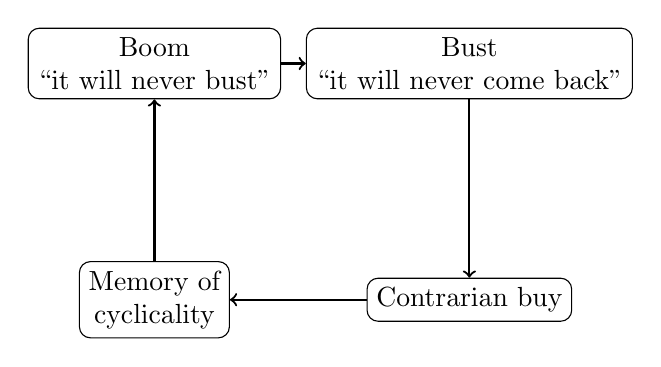
\begin{tikzpicture}[scale=1]
\node[draw, rounded corners, align=center] (boom) at (0,2) {Boom\\``it will never bust''};
\node[draw, rounded corners, align=center] (bust) at (4,2) {Bust\\``it will never come back''};
\node[draw, rounded corners, align=center] (buy) at (4,-1) {Contrarian buy};
\node[draw, rounded corners, align=center] (memory) at (0,-1) {Memory of\\cyclicality};
\draw[->, thick] (boom) -- (bust);
\draw[->, thick] (bust) -- (buy);
\draw[->, thick] (buy) -- (memory);
\draw[->, thick] (memory) -- (boom);
\end{tikzpicture}
\end{center}
\end{figure}

That is the first genuinely formal structure in the lecture: not a formula, but a repeatable decision rule. The speaker later reports that he made a little over \(\$40\) million in one year. We keep that number as a claim of scale, but the deeper lesson lies in the relation between sentiment and action.

\paragraph{Worked example.} The lecture becomes mathematically explicit when the speaker recounts his first serious distressed-debt purchase. He says he maxed out a credit card at \(\$70{,}000\), bought a package of failed-loan assets with face value \(\$1.6\) million, and paid \(\$64{,}000\) for it. If we write
\[
F=\$1.6\times 10^6,
\qquad
P=\$64{,}000,
\]
then the paid fraction of face is
\begin{align}
d &= \frac{P}{F}
   = \frac{64{,}000}{1.6\times 10^6}
   = 0.04,\\
\delta &= 1-d = 0.96.
\end{align}
So the package was purchased at about \(4\%\) of face, or at about a \(96\%\) discount. The lecture does not convert this into a general pricing theory. Instead it binds the arithmetic to emotion. The speaker says he felt sick after making the trade, called an older friend, and was told that the first deal is the hardest and will never feel this bad again. The arithmetic alone does not carry the lesson. The lesson is that uncertainty remains part of the mechanism.

The section then widens. Asked what industry people should get into now, the speaker answers: something where they have an edge. If everyone already agrees it is a great idea, the price has adjusted and the opportunity has largely disappeared. Again the lecture privileges contrarian timing and local advantage over generic enthusiasm.

A personal axis is added next. The speaker says everybody doubted him except his wife. Then he explicitly distinguishes being rich from having a good life. Money is part of it, but only part. This matters because the lecture is beginning to braid money, marriage, faith, and uncertainty into a single architecture.

\subsection{Question \& Answer}

\paragraph{Question.} How are we supposed to plan a life when the future is uncertain?

\paragraph{Answer.} The lecture answers by replacing drift with backward construction. We are asked to think about where we want to be in \(30\) years, form a broad picture, and then work backward to determine what should be done now. In compact form, we may write
\begin{equation}
A_0 = \mathcal{R}(T_{30}),
\end{equation}
where \(T_{30}\) denotes the rough target state \(30\) years out, \(A_0\) denotes present action, and \(\mathcal{R}\) stands for reverse engineering. This notation is ours, not the speaker's, but it captures the structure of the advice faithfully.

The lecture's planning rule is procedural:
\begin{enumerate}
\item Choose a broad end state \(T_{30}\).
\item Infer the milestones that would have to exist if that end state were to become real.
\item Choose present action \(A_0\) so those milestones become reachable.
\end{enumerate}

The speaker compares this to knowing what will be on a test. If one knows the target, preparation becomes more obvious. The point is not prediction. The point is deliberateness.

\section{Recovery, Character, and Hiring Weakness}

At this point the lecture changes register sharply. The next interview begins not with inherited privilege or even cyclical investing, but with a federal penitentiary. The narrative disruption matters. It broadens the lecture's map of who can build wealth and from what starting point.

\paragraph{Anecdote.} The interviewee says he spent almost four years in prison. He also says that his family runs an HVAC company, \(42\) years old, originally in the Tulsa area, later expanded into Texas. He reports a \(49\%\) exit roughly six months earlier, says the business sold at \(7\times\) what they had into it, and places Oklahoma revenue at about \(\$3.5\) million. The host summarizes this as roughly \(\$20\) million of value created.

\begin{remark}
The numerical content in this segment is suggestive rather than closed. We retain the reported \(49\%\) exit, \(7\times\) multiple, \(\$3.5\) million revenue, and host-side \(\$20\) million estimate, but we do not force them into a complete valuation identity that the transcript itself does not provide.
\end{remark}

\paragraph{Claim.} Asked what brought him back from rock bottom, the speaker attributes the turnaround to his relationship with Jesus Christ. That faith claim belongs to the explanatory structure of the interview and should remain visible as such. It is not auxiliary color; it is presented as the primary account of recovery.

\paragraph{Mechanism.} The business lesson comes next, and here the lecture returns to a theme already present in Keller's remarks: one must not fear stronger people. A former cellmate, previously an executive at Procter \& Gamble, gave him a compact rule: hire your weakness. Strength is where one makes money; weakness is where one keeps it or loses it.

The sentence is not algebra, but it has an algebraic form. Profit originates where one is strong. Preservation depends on whether one's blind spots are corrected by people who are better than oneself in precisely those places. The lecture is pushing us toward an organizational view of character: strength is not enough if it is surrounded by unmanaged weakness.

The prison story also adds a more elemental human observation. When nobody has anything, the speaker says, then one sees what people really are, because there is nothing to trade except handshake, loyalty, and care. In the architecture of the lecture this becomes a bridge between moral testimony and commercial method. Trust is not outside business. It is one of the few things that survives when other resources disappear.

\section{Corporate Entrepreneurship and the Three-Part Survival Rule}

After a promotional interruption, the lecture restarts at a different scale. Jim Keyes enters not as a small operator but as a corporate executive associated with 7-Eleven and Blockbuster. This section matters because it complicates the earlier doctrine that wealth must come only from founding and owning from scratch.

\paragraph{Anecdote.} Keyes says he sold 7-Eleven for many billions of dollars and describes a childhood in a house with no running water. The lecture again binds very large outcomes to humble beginnings, but now it does so inside the corporate world.

\paragraph{Claim.} Asked what the most successful CEOs have in common, he answers: fearlessness. Not theatrical fearlessness, but the ability to walk up, transact, and act without paralysis. He then adds a second principle: relationships are everything, because the most valuable resource in any company is the human resource.

\begin{definition}
A \emph{corporate entrepreneur}, in the language of this lecture, is a person who behaves entrepreneurially inside a larger institution. The structure is greater, the exposure is different, but initiative, judgment, and execution still determine outcome.
\end{definition}

This is the lecture's answer to a real objection. Not everybody is suited for naked entrepreneurial uncertainty. Some people need the scaffolding of the corporate form. The lecture does not deny that. It reframes the issue. One can still create value inside structure if one behaves as an entrepreneur rather than as a passenger.

\subsection{Question \& Answer}

\paragraph{Question.} Can one become wealthy without being a pure founder?

\paragraph{Answer.} In the logic of this lecture, yes. The corporate world can still reward entrepreneurial conduct, but only if one does not use structure as an excuse for passivity. The institution gives support; it does not remove the need for initiative.

The section reaches its most compact form when Keyes gives what is essentially a three-part operating theorem.

\begin{proposition}
Business survival, in Keyes's formulation, rests on three coupled terms:
\begin{equation}
\{\text{cash},\ \text{communications},\ \text{character}\}.
\end{equation}
Cash is oxygen, communications create alignment, and character determines whether the enterprise survives stress.
\end{proposition}

\begin{figure}
\begin{center}
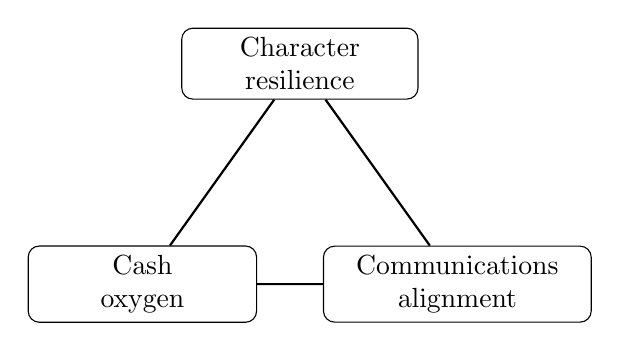
\begin{tikzpicture}[scale=1]
\node[draw, rounded corners, minimum width=2.9cm, align=center] (cash) at (0,0) {Cash\\oxygen};
\node[draw, rounded corners, minimum width=3.4cm, align=center] (comm) at (4,0) {Communications\\alignment};
\node[draw, rounded corners, minimum width=3.0cm, align=center] (char) at (2,2.8) {Character\\resilience};
\draw[thick] (cash) -- (comm) -- (char) -- (cash);
\end{tikzpicture}
\end{center}
\end{figure}

The lecture unpacks the triad carefully. Cash flow must be watched through debt, payables, and receivables because businesses suffocate before they philosophize. Communications matter because frightened or confused teams cannot execute. Character matters because bad times test values, resilience, and self-confidence. This is the lecture's closest approach to a theorem, and it should be preserved in that shape.

The closing turn in this section is unexpectedly literary. Asked which book most changed his business life, Keyes names the \emph{Boy Scout Handbook}. He then recites the familiar virtues: trustworthy, loyal, helpful, friendly, courteous, kind, obedient, cheerful, thrifty, brave, clean, reverent. The lecture is doing something subtle here. It is taking a large-scale executive framework and grounding it in a moral vocabulary simple enough to memorize.

\section{Time, Culture, Sacrifice, and Choosing a Life}

The final major movement begins with spectacle: a private jet on a Dallas tarmac. But the lecture uses the spectacle only as an entry point. Almost immediately the jet becomes a question about time, not merely status.

\paragraph{Anecdote.} Ben Pogue says his last commercial flight was in \(2018\), that he now flies roughly \(300\) hours, and that the plane is mostly used for personal travel, family movement, and what he calls a more eclectic learning environment for his children. He reports that a new aircraft of this kind would be around \(\$50\) million, that he put about \(\$5\) million into interior and paint, and that his all-in basis was ``probably about'' \(\$20\) million.

\begin{remark}
The accounting in this portion of the lecture is conversational and partly garbled. We keep the numbers \(\$50\) million, \(\$5\) million, and \(\$20\) million as reported claims, but we do not force them into an exact balance-sheet reconstruction.
\end{remark}

What matters for the lecture is not primarily the purchase price. It is the conversion rule the speaker gives for private flight: money cannot create more hours, but it can sometimes recover time that would otherwise be consumed. The jet is thus framed as a tool that buys back schedule rather than as a magical source of earnings.

That thought leads smoothly into business. Pogue says his main company was a second-generation construction business, taken over in \(2009\) and bought fully in \(2016\). Asked how he stood out in a competitive field, he answers in a way now familiar to us: by going all in on people and culture. Every company, he says, is in the people business and the service business, whether it knows it or not.

\paragraph{Mechanism.} The lecture here links care, standards, and performance. People will run through walls, the speaker says, if they know you care for them and will be there for them. The point is not sentimental. It is organizational. High expectations become productive only when trust exists on both sides.

A further sharpened principle then appears. One must not merely avoid losing. One must play to win. The speaker explicitly resists defensive box-checking and later extends that same logic to investment: diversified portfolios may be suitable for safety, but the wealthiest people he has observed often concentrated heavily into one or two things and executed those bets well.

The numerical scale of the section is stated plainly:
\begin{align}
R_{\text{personal,max}} &\approx \$200\times 10^6 \quad \text{in one year},\\
V_{\text{company}} &\approx \$1.5\times 10^9 \quad \text{in volume}.
\end{align}
These are reported interview figures, not audited filings, but they matter because they anchor the later questions about sacrifice.

Once scale is established, the lecture turns darker. Success, the speaker says, often costs friends, relationships, and even family proximity. He distinguishes those who cheer for you through everything from mere blood relation. Then he recounts the hardest period of his life: an unexpected divorce in \(2012\), with very young children, and the collapse that followed.

The host uses this low point to raise a question that the lecture has been circling for some time: if business is a long-horizon game, what does it require from marriage? The answer is direct. One must choose with extraordinary care. Chemistry and attraction matter, but kindness, selflessness, ease, commitment, and alignment of faith matter more for long-run stability. In the architecture of the lecture, spouse selection is not outside business method. It is one of the conditions under which sustained business effort becomes possible.

The section closes in the same register. Faith is not treated as private ornament but as the speaker's account of what held when other things fell away. The final advice is correspondingly broad: do not sweat small things, do not put limits on what God may intend for your life, and do not confuse present planning with total authorship of the future.

\section{Summary}

This lecture never yields a single clean theorem of wealth, and it would be unfaithful to force one upon it. What it does yield is a recurring set of structures. Business ownership appears again and again as the preferred site of wealth formation. People, incentives, and culture are treated as multiplicative forces rather than decorative virtues. Concentration is favored over early dispersion, but only in the form of mastery rather than mere recklessness. Cycles reward those who remember the opposite phase. Cash, communications, and character determine whether an enterprise survives its bad times. And beneath all of this runs a longer argument: time horizon, spouse choice, faith, and the ability to live with uncertainty are not side issues. They are part of the same architecture as profit and scale.

In that sense the lecture's method is the lesson. We begin with a raw question in the street, and by the end we have not one answer but a field of linked principles: build something irresistible, hire stronger people, endure the first hard deal, reverse engineer the future, correct weakness through others, guard cash, communicate clearly, keep character in bad times, and spend money only where it genuinely buys back freedom.